\chapter{Introduction to OpenFOAM\textsuperscript{\textregistered}}

\label{openfoam}

OpenFOAM\textsuperscript{\textregistered} is a Free Open Source Software (FOSS) where we can get the source code along with binary executable for all the solvers. The FOAM project (precursor to OpenFOAM\textsuperscript{\textregistered}) was created at Imperial College London in the late 80s and early 90s by Henry Weller, along with Hrvoje Jasak, using the new object-oriented programming language C++. Succeeding the commercial software FOAM, OpenFOAM\textsuperscript{\textregistered} was released in 2004 as free and open-source software under the GNU General Public License (GPL), a widely used free software license, which guarantees end users the freedom to run, study, share and modify the software.

OpenFOAM\textsuperscript{\textregistered} has been used instead of ANSYS\textsuperscript{\textregistered} \textit{Fluent} because it has many potential advantages. Here we can modify the existing solvers/models to suit our particular needs, compile them and add them to our library. One distinguishing feature of OpenFOAM\textsuperscript{\textregistered} is its syntax for tensor operations and partial differential equations (PDEs) that closely resembles the equations being solved. For example, the equation: 
\begin{equation}
\dfrac{\partial(\rho U)}{\partial t} + \nabla \boldsymbol{\cdot} \phi U - \nabla \boldsymbol{\cdot} \mu \nabla U = - \nabla p
\end{equation}
is represented by the code: 
\begin{verbatim}
Solve
(
	fvm :: ddt(rho,U)
	+ fvm :: div(phi,U)
	- fvm :: laplacian(mu,U)
	==
	-fvc :: grad(p)
);

\end{verbatim}

Thus we can see that all the mathematical operators like divergence, curl, gradient, laplacian etc. are well defined in OpenFOAM\textsuperscript{\textregistered}. OpenFOAM\textsuperscript{\textregistered} treats fluid, structural, thermal or acoustic or any other field problems in the exactly same way as long as there are governing equations in them and they can be written in conservative form. It uses finite volume discretization method. Whenever we are programming any new solver, 90 percent of the code remains same with baseline solver and changes to be made are less than 10 percent. Thus using OpenFOAM\textsuperscript{\textregistered}, There is no need to write the entire code right from scratch every time. We can just edit the existing solver and save lot of time.

Automatic mesh generation utility called \textit{SnappyHexMesh} comes along with OpenFOAM where in we have to give .stl or .obj file of geometry and specify the level of refinement needed. The rest is taken care by it. This is particularly useful when we have to couple CFD analysis to the optimizer. \textit{SnappyHexMesh} is still in development phase and is getting better with every release.

The absence of Graphical User Interface (GUI) can be taken as an advantage because we come to know the actual physics of flow happening behind the scene. If you become moderately expert in OpenFOAM\textsuperscript{\textregistered} then it saves a lot of time because we can programatically control all the inputs/outputs and we can automate many processes right from mesh generation to post processing.

OpenFOAM\textsuperscript{\textregistered} comes with a Open Source CFD post processing utility known as \textit{ParaView}.\textit{ParaView} accepts both point field data as well as volume field data. Since we solve Navier Stokes equations using Finite Volume Approach, at the end we are provided with data at the centre of cells. In this case, \textit{ParaView} is very useful. On the other hand, \textit{Tecplot\textsuperscript{\textregistered}} (commercially available CFD post software) accepts data only at the vertices.

\section{OpenFOAM\textsuperscript{\textregistered} for CFD researchers}

The main difficulty for engineers in using OpenFOAM\textsuperscript{\textregistered} is that it is not user friendly. Learning curve for openFOAM\textsuperscript{\textregistered} is very steep. But learning it adds value to one's skill set. OpenFOAM\textsuperscript{\textregistered} is used in the cases where ANSYS\textsuperscript{\textregistered} \textit{Fluent} fails. Because it has the transparency within it. It is arguably equally powerful as ANSYS\textsuperscript{\textregistered} \textit{Fluent}. To do any simulation using OpenFOAM\textsuperscript{\textregistered}, We have to basically think all the way back from vector Calculus to advanced topological errors. This will not only make us think like a computational scientist but will create awareness about how do we go about solving a problem from its inception to execution.



 

There are also many graphical user interfaces available for OpenFOAM\textsuperscript{\textregistered}. However using gui, we can do only limited tasks. OpenFOAM\textsuperscript{\textregistered} also comes with many utilities using which we can convert mesh generated by third party meshing tools like ANSYS\textsuperscript{\textregistered} \textit{Gambit}, \textit{Gmsh}, etc to OpenFOAM\textsuperscript{\textregistered} format.

OpenFOAM\textsuperscript{\textregistered} also comes with parallel processing utilities using which we can decompose, reconstruct and redistribute the computational case to perform parallel calculations, at times better than other CFD software. All these things makes OpenFOAM\textsuperscript{\textregistered} suitable for general engineers because we come to know whats happening behind the screen rather than just clicking the buttons. 


\section{Computational mesh generation using \textit{SnappyHexMesh}}

\textit{SnappyHexMesh} is a hexahedral unstructured mesh generation tool included in the distribution of OpenFOAM\textsuperscript{\textregistered}. \textit{SnappyHexMesh} can use a 3-D .stl surface and iteratively build a mesh upon it. Some options allow construction of several cell layers of a controllable height above the 3D surface.This feature makes it possible to have a refined mesh in the region of high velocity gradients, close to the surface.  Near the surface, the mesh is refined and cells are splitted acoordingly. The process is explained in Figure ~\ref{Snappy Hex Mesh} .Several regions can be selected to be refined to a desired level, and this method creates mesh of a cell aspect ratio close to 1.This is done in order to ensure that OpenFOAM\textsuperscript{\textregistered} can solve the numerical problems with the highest efficiency and accuracy using meshes generated with \textit{SnappyHexMesh}. The meshing tool \textit{SnappyHexMesh} can be run in parallel on a computer cluster or a PC.

\begin{figure}[htbp]
	\centering
	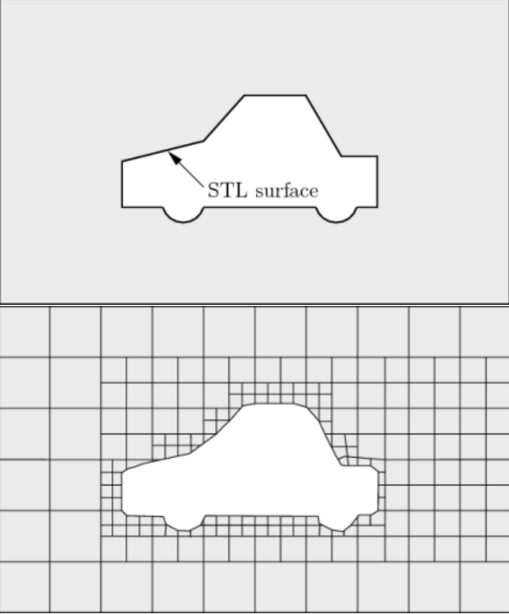
\includegraphics[width=200 pt]{mesh/snappyHexMesh.png}
	\caption{Surface snapping process in \textit{snappyHexMesh} }
	\label{Snappy Hex Mesh} %      only if needed
\end{figure} 

Although in the Figure ~\ref{Snappy Hex Mesh}, it is shown for 2D, \textit{SnappyHexMesh} is a 3D meshing utility.

\section{Validation of OpenFOAM\textsuperscript{\textregistered} CFD results}
\label{results}

This section describes the values of $C_{DV}$ obtained for four standard axisymmetric LTA envelope shapes, viz., GNVR \cite{Ram}, NPL \cite{cheeseman2012} Zhiyuan-1 \cite{zhiyuan}, and Wang \cite{Wangshape}, using OpenFOAM\textsuperscript{\textregistered}, and a comparison with the quoted values. 
Fig. \ref{All profiles} shows these four profiles. All the simulations were carried at zero degree angle of attack.

\begin{figure}[H]
	\centering
	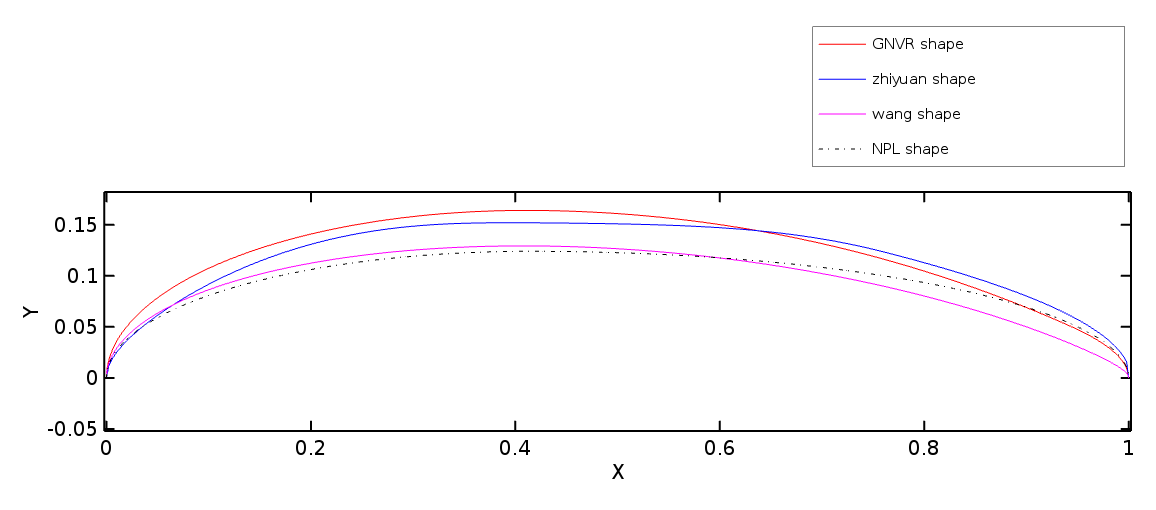
\includegraphics[width=400 pt]{rnd/all_profiles.png}
	\caption{Four standard shapes available in literature}
	\label{All profiles} 
\end{figure}
The specifications of machine, operating system, and software used in this study are as follows:
\begin{itemize}
	\item Model name = Intel(R) Xeon(R) CPU E5-2650
	\item Number of physical cores = 40
	\item Processor speed = 2.8 GHz
	\item Operating system = Cent OS 7.4
	\item OpenFOAM\textsuperscript{\textregistered} version = 4.1
\end{itemize}
Following subsections shows flow conditions, solver parametres and results of CFD simulation carried on the above mentioned standard shapes. 

\subsection{GNVR shape \cite{Ram}}
The GNVR shape \cite{Ram} is named after late Prof. G.N.V Rao of Indian Institute of Science, Bengaluru. It consists of three standard geometrical constructs, viz, ellipse, circle and parabola. The entire envelope shape is parametrized in terms of its maximum diameter ($D$), as follows:
\begin{center}
	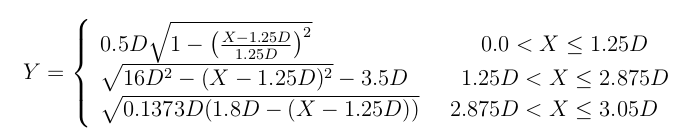
\includegraphics[width= 200 pt]{rnd/GNVR_equations.png}
\end{center}
Fig. \ref{prismlayers} shows the mesh near the surface of GNVR shape to resolve the boundary layer.
\begin{figure}[H]
	\centering
	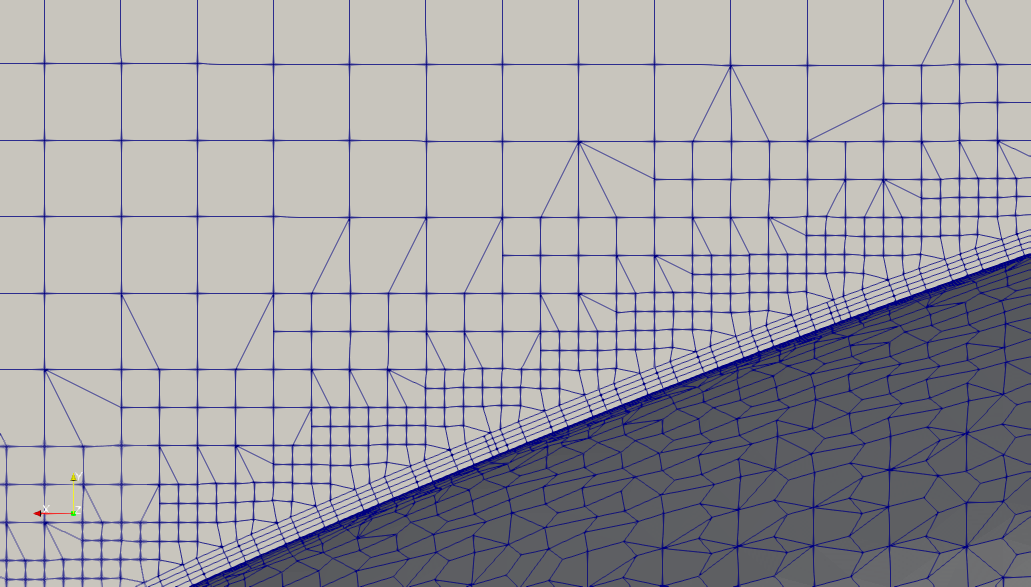
\includegraphics[width=300 pt]{rnd/prism_layer.png}
	\caption{Prism layers on the surface of GNVR to capture boundary layer}
	\label{prismlayers} %      only if needed
\end{figure}


The flow conditions used for the simulation are similar to that of Kanikdale et al. \cite{Kanikdale}. Taking advantage of the axisymmetric nature of GNVR shape, its 3D CFD analysis was carried out only for 1/4 of its shape. The flow conditions and solver parameters are shown in Table \ref{Flow conditions and solver parametres for GNVR shape}

\begin{table}[H]
	\caption{Flow conditions and solver parametres for GNVR shape}
	\label{Flow conditions and solver parametres for GNVR shape}
	\centering
	\begin{tabular}{ll}
		\hline \hline
		Flow Conditions & Solver parametres  \\ \hline \hline
		
		$ Velocity = 50.339 \; m/s$ & $Number \; of \; cells = 646,639$    \\  
		$ Pressure = 101325 \; Pa $ & $ Number \; of \; parallel \; cores = 20 $     \\
		$ Density = 1.225 \; kg/m^{3} $ & $ Time \; taken \; for \; solution = 475~s  $    \\
		$ Reynolds \; number = 34.783 * 10^{6} $ &    \\
		$ Turbulence \; model = k - \epsilon $ &     \\
		\hline
	\end{tabular}
	%	\end{ruledtabular}
\end{table}





The variation of Pressure coefficient ($C_{P}$) along the envelope length obtained using OpenFOAM\textsuperscript{\textregistered} is compared with that of using ANSYS\textsuperscript{\textregistered} \textit{Fluent} by Kanikdale et al. \cite{Kanikdale} and Panel method by Narayana and Srilatha \cite{srilata}. 

\begin{figure}[H]
	\centering
	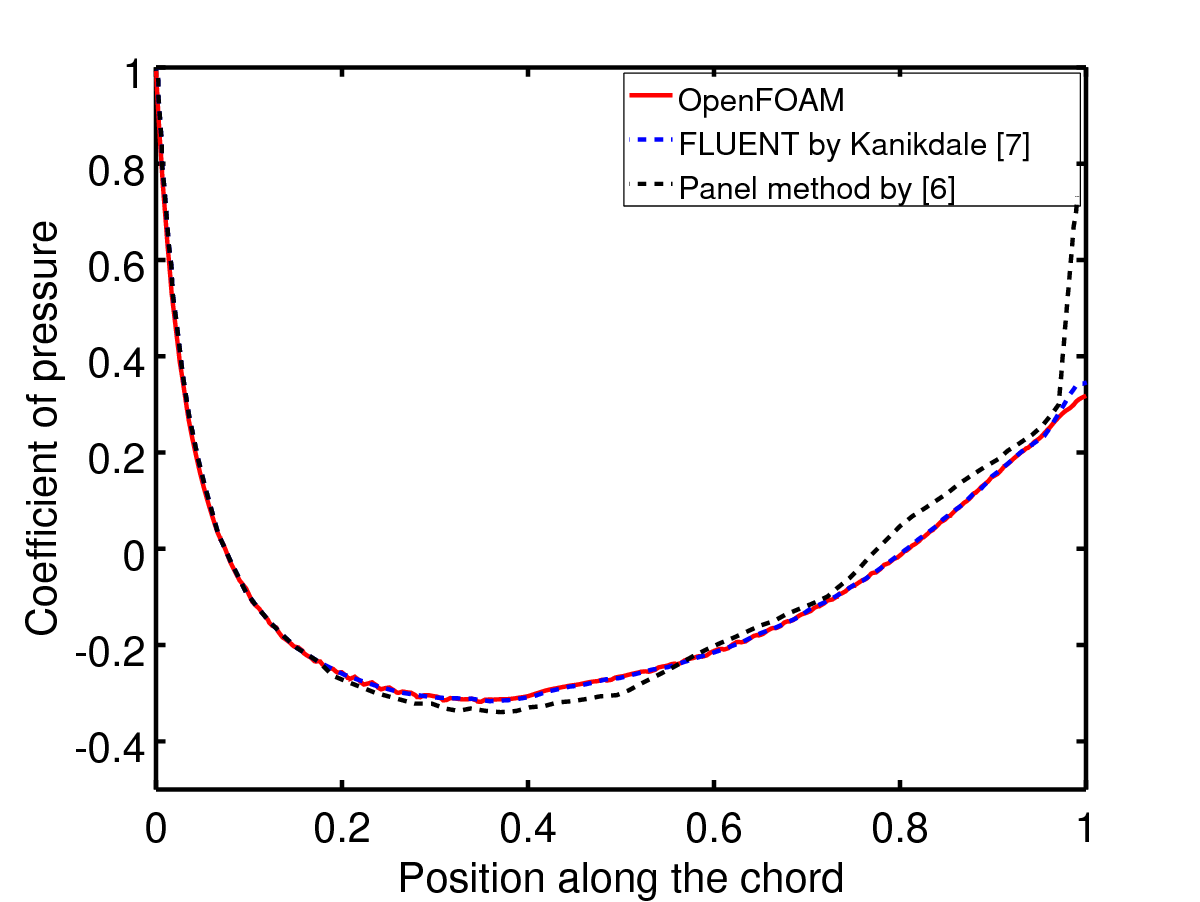
\includegraphics[width=270 pt]{rnd/GNVR_cp.png}
	\caption{$C_{P}$ distribution for GNVR profile obtained by OpenFOAM\textsuperscript{\textregistered}, Source Panel Method \cite{srilata} and ANSYS\textsuperscript{\textregistered} \textit{Fluent} \cite{Kanikdale}}
	\label{fig:GNVR pressure distribution} %      only if needed
\end{figure}

It can be observed from Fig. \ref{fig:GNVR pressure distribution} that the $C_{P}$ distribution obtained by OpenFOAM\textsuperscript{\textregistered} matches well with that obtained by ANSYS\textsuperscript{\textregistered} by Kanikdale et al. \cite{Kanikdale} along the entire envelope length, except at the trailing edge, where the flow is separated. The distribution obtained by Panel Method \cite{srilata} shows very high pressure recovery at trailing edge because attached flow is assumed, and the \textit{Kutta} condition is satisfied.

\subsection{Zhiyuan-1 shape \cite{zhiyuan}}

The equation that define the Zhiyuan-1 shape is:
\begin{center}
	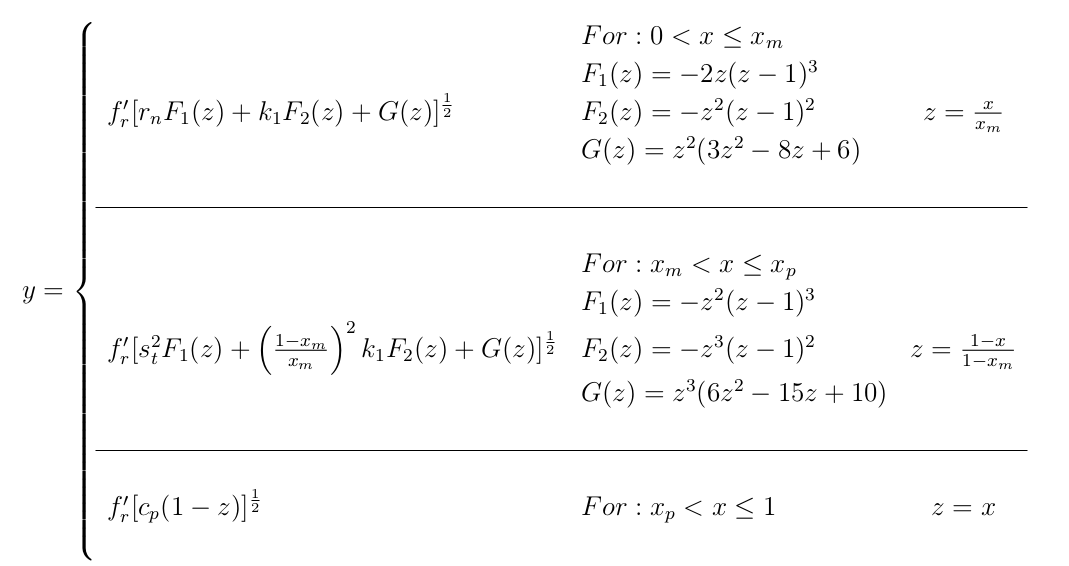
\includegraphics[width= 400 pt]{rnd/zhiyuan_equations.png}
\end{center}
Values of the constants mentioned above are as follows:

$ x_{m} = 0.393591, \quad x_{p} = 0.7570323,\quad r_{n} = 0.5070992,\quad k_{1} = 0.291256,\quad c_{p} = 2.735107,\quad f_{r}^{'} = 0.1515518 \quad and \quad  s_{t} = 3.236105 $


Suman et al. \cite{suman} carried out a Reynolds-Averaged Navier - Stokes (RANS) simulation to reproduce the results obtained by Wang et al. \cite{zhiyuan} for transition assumed at the leading edge itself, i.e., for a fully turbulent flow. They have also obtained results for various assumed locations of the transition points, resulting in pockets of laminar and turbulent regions in the computational domain.\\
In the present study, a 3-D CFD analysis for Zhiyuan-1 shape was carried out and pressure distribution is shown in Fig. \ref {fig:Zhiyuan-1 pressure}. 
\begin{figure}[H]
	\centering
	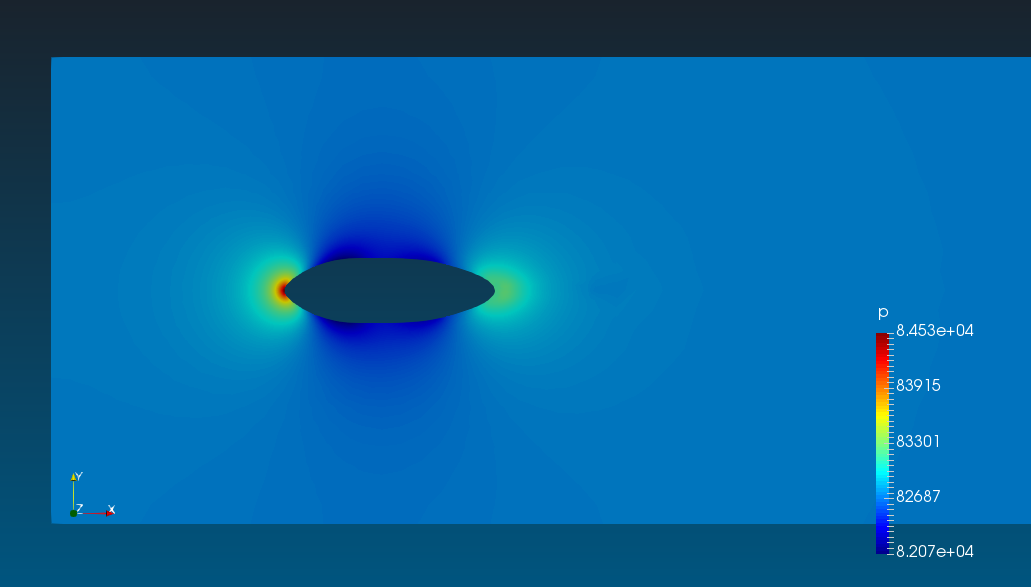
\includegraphics[width=300 pt]{rnd/pressure_zhiyuan.png}
	\caption{Pressure distribution on Zhiyuan-1 airship shape}
	\label{fig:Zhiyuan-1 pressure} %      only if needed
\end{figure}

The results were obtained only for one half of the envelope and `SymmetryPlane' boundary condition was incorporated for the other half to reduce the computational time.

The flow conditions used for the simulation were same as used by Suman et al. \cite{suman} and Wang et al. \cite{zhiyuan} and is given in Table \ref{Flow conditions and solver parametres for Zhiyuan-1 shape}

\begin{table}[H]
	\caption{Flow conditions and solver parametres for Zhiyuan-1 shape}
	\label{Flow conditions and solver parametres for Zhiyuan-1 shape}
	\centering
	\begin{tabular}{ll}
		\hline \hline
		Flow Conditions & Solver parametres  \\ \hline \hline
		
		$ Velocity = 60.39 \; m/s$ & $Number \; of \; cells = 2,982,639$    \\  
		$ Pressure = 101325 \; Pa $ & $ Number \; of \; parallel \; cores = 8 $     \\
		$ Density = 1.225 \; kg/m^{3} $ & $ Time \; taken \; for \; solution = 4534 \; s  $    \\
		$ Reynolds \; number = 2.4 * 10^{6} $ &    \\
		$ Turbulence \; model = \kappa \omega \; SST $ &     \\
		\hline
	\end{tabular}
	%	\end{ruledtabular}
\end{table}


Fig. \ref{Zhiyuan_OF_RANS} shows a comparison between the $C_{P}$ distribution for Zhiyuan-1 envelope shape using  OpenFOAM\textsuperscript{\textregistered} with ANSYS\textsuperscript{\textregistered} \textit{Fluent} and experimental results quoted by Wang et al. \cite{zhiyuan}
\begin{figure}[H]
	\centering
	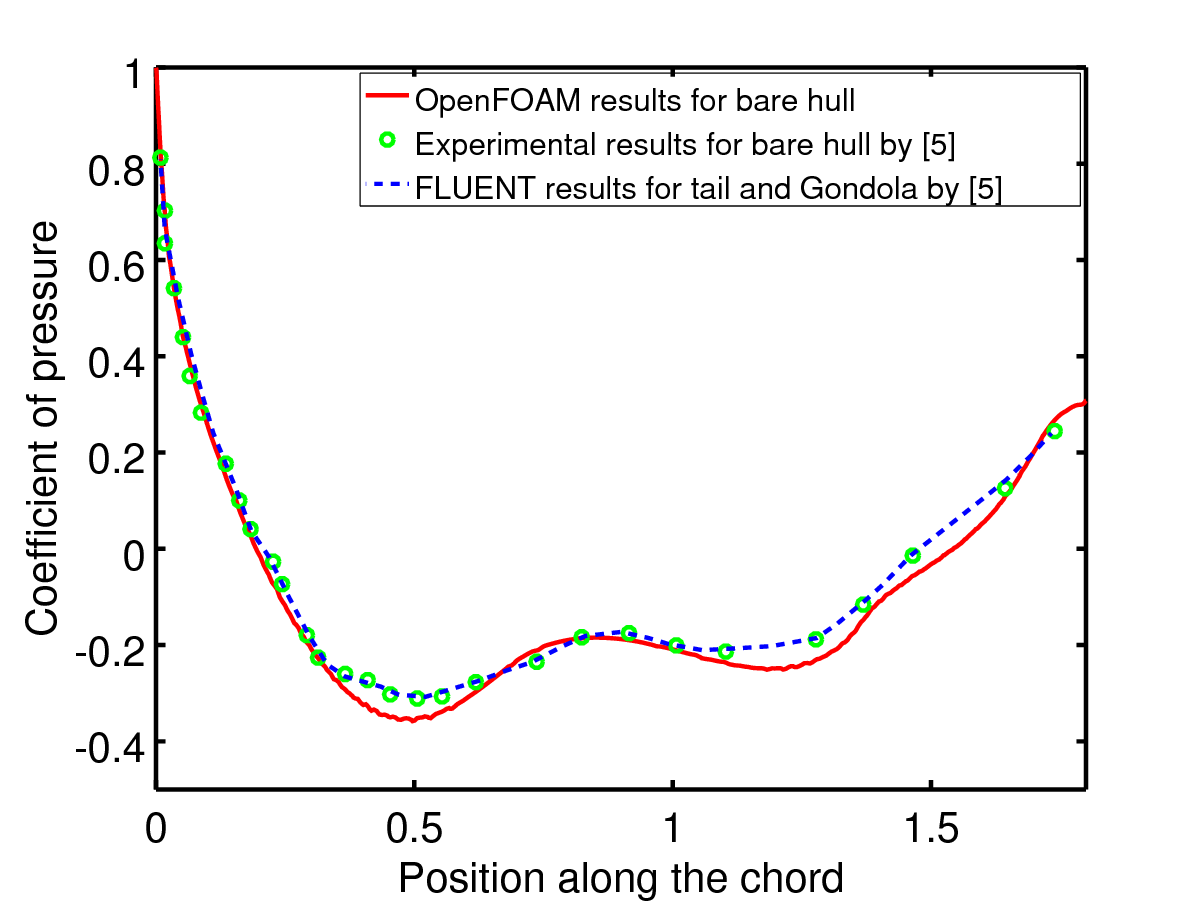
\includegraphics[width=270 pt]{rnd/zhiyuan_cp.png}
	\caption{$C_{P}$ distribution for Zhiyuan-1 shape using OpenFOAM\textsuperscript{\textregistered}, Experiments \cite{zhiyuan} and ANSYS\textsuperscript{\textregistered} \textit{Fluent} \cite{zhiyuan}}
	\label{Zhiyuan_OF_RANS} %      only if needed
\end{figure}

Table \ref{Zhiyuan -1 Cdv} compares the components of $C_{DV}$ obtained using OpenFOAM\textsuperscript{\textregistered} and RANS \cite{suman}.

\begin{table}[H]
	\centering
	\caption{\label{Zhiyuan -1 Cdv} Comparison of OpenFOAM\textsuperscript{\textregistered} results with RANS \cite{suman} for Zhiyuan -1 shape}
	%\begin{ruledtabular}
	\begin{tabular}{cccc}
		\hline \hline
		& OpenFOAM\textsuperscript{\textregistered} & RANS \cite{suman} & \% error    \\ \hline \hline
		
		$ C_{DV} (Viscous)$ & 0.01989 & 0.01890 & 5.3    \\  
		$ C_{DV} (Pressure) $ & 0.00583 & 0.00568 & 2.8    \\
		$ C_{DV} (Total) $ & 0.02573 & 0.02456 & 4.8    \\  \hline
	\end{tabular}
	%	\end{ruledtabular}
\end{table}


\subsection{Wang Shape \cite{Wangshape}}
Wang et al. \cite{Wangshape} proposed a new shape exploring the better shapes in the view of multi-disciplinary optimization. The geometry is defined by five shape parameters namely \textit{a, b, c, d} and length \textit{l}. The original equation proposed by Wang et al.\cite{Wangshape} is given by Eq. \ref{wang_eqn}:
\begin{equation}
64(y^{2} + z^{2}) = a(l-x)\left( bx - l \sqrt{c} + \sqrt{c l^{2} - dlx} \; \right) 
\label{wang_eqn}
\end{equation}

The values taken for the parameters of Wang shape are as follows: \\
\quad \textit{a = 7.447  \quad b = 2.072  \quad  c = 9.010 \quad d = 7.981} \quad and \quad \textit{l = 194.0} \\

For the sake of convenience, geometry is scaled down by length (\textit{l}) in all directions.
Wang shape defined by Eq. \ref{wang_eqn} is a body of revolution and also can be obtained by rotating the profile given by Eq. \ref{wang_eqn_2} through $ 360^{o} $.
\begin{equation}
y = \dfrac{\sqrt{a(l-x)\left( bx - l \sqrt{c} + \sqrt{c l^{2} - dlx} \; \right)}}{8} 
\label{wang_eqn_2}
\end{equation}

The flow conditions and solver parameters used for the simulation are shown in Table \ref{Flow conditions and solver parametres for Wang shape}:

\begin{table}[H]
	\caption{Flow conditions and solver parametres for Wang shape}
	\label{Flow conditions and solver parametres for Wang shape}
	\centering
	\begin{tabular}{ll}
		\hline \hline
		Flow Conditions & Solver parametres  \\ \hline \hline
		
		$ Velocity = 51 \; m/s$ & $Number \; of \; cells = 1,060,202$    \\  
		$ Pressure = 8750 \; Pa $ & $ Number \; of \; parallel \; cores = 8 $     \\
		$ Density = 1.225 \; kg/m^{3} $ & $ Time \; taken \; for \; solution = 2865 \; s  $    \\
		$ Reynolds \; number = 3.01 * 10^{6} $ &    \\
		$ Turbulence \; model = Spalart Allmaras $ &     \\
		\hline
	\end{tabular}
	%	\end{ruledtabular}
\end{table}


The values obtained for finer grid case using OpenFOAM\textsuperscript{\textregistered} are compared with those of using ANSYS\textsuperscript{\textregistered} \textit{Fluent}. Fig. \ref{wang comp} shows the comparison of $ C_{P} $ distribution.
\begin{figure}[H]
	\centering
	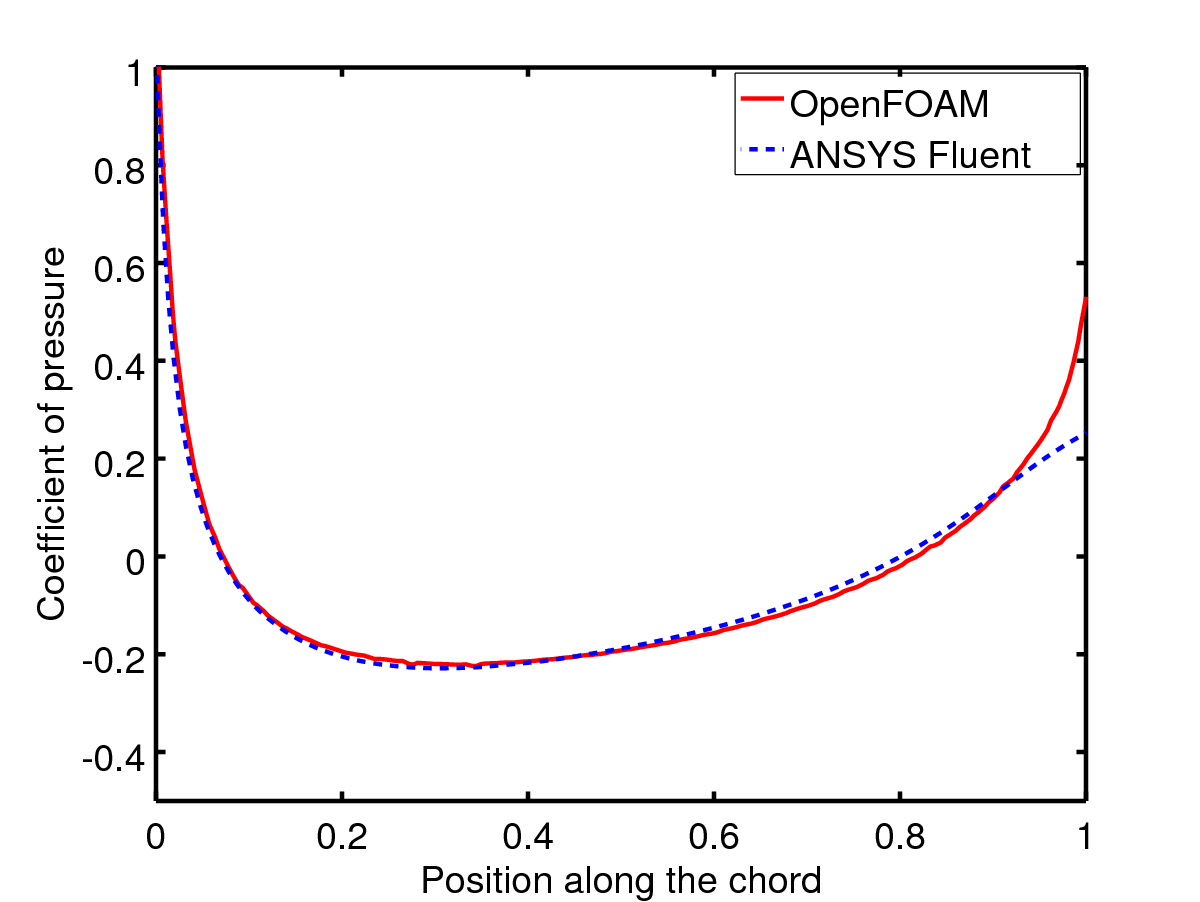
\includegraphics[width=300 pt]{rnd/wang_cp.png}
	\caption{Comparison of OpenFOAM\textsuperscript{\textregistered} results with ANSYS\textsuperscript{\textregistered} \textit{Fluent} results for pressure distribution of Wang shape}
	\label{wang comp} %      only if needed
\end{figure}

Table \ref{wang table} shows the comparison of $ C_{DV} $ obtained using OpenFOAM\textsuperscript{\textregistered} and ANSYS\textsuperscript{\textregistered} \textit{Fluent}

\begin{table}[H]
	\centering
	\caption{\label{wang table} Comparison of OpenFOAM\textsuperscript{\textregistered} results with ANSYS\textsuperscript{\textregistered} \textit{Fluent} for Wang shape}
	%	\begin{ruledtabular}
	\begin{tabular}{cccc}
		\hline \hline
		& OpenFOAM\textsuperscript{\textregistered} & ANSYS\textsuperscript{\textregistered} \textit{Fluent} & \% error \\ \hline \hline
		
		$ C_{DV} $ & 0.02730 & 0.02610 & 4.6    \\ \hline
	\end{tabular}
	%	\end{ruledtabular}
\end{table}


\subsection{NPL Shape \cite{cheeseman2012}}
NPL shaped envelope is basically the combination of two half prolate joint at maximum diameter. It is known for its lower drag characteristics. The mathematical representation of prolate is:
\begin{equation}
\frac{x^{2}}{a^{2}} + \frac{y^{2}}{b^{2}} + \frac{z^{2}}{c^{2}} = 1
\label{NPL_eqn}
\end{equation}
The same surface given by Eq.\ref{NPL_eqn} can also be obtained by rotating the curve given by Eq.\ref{NPL_eqn_2} along X axis
\begin{equation}
y = \begin{cases}
\pm b \sqrt{1-\dfrac{(x-a)^{2}}{a^{2}}} & When \; x \le a \\
\pm b \sqrt{1-\dfrac{(x-a)^{2}}{2a^{2}}} & When \; x \le a
\end{cases}
\label{NPL_eqn_2}
\end{equation}

Values of constants mentioned above are: \textit{a = 82.485  \quad and \quad b = 24.681  }

For the sake of convenience, The surface generated is scaled down by length (\textit{l}) in all directions.The values obtained for finer grid case using OpenFOAM\textsuperscript{\textregistered} are compared with those of using ANSYS\textsuperscript{\textregistered} \textit{Fluent}. 

The flow conditions and solver parameters used for the simulation are shown in Table \ref{Flow conditions and solver parametres for NPL shape}

\begin{table}[H]
	\caption{Flow conditions and solver parametres for NPL shape}
	\label{Flow conditions and solver parametres for NPL shape}
	\centering
	\begin{tabular}{ll}
		\hline \hline
		Flow Conditions & Solver parametres  \\ \hline \hline
		
		$ Velocity = 51 \; m/s$ & $Number \; of \; cells = 1,063,736$    \\  
		$ Pressure = 87500 \; Pa $ & $ Number \; of \; parallel \; cores = 8 $     \\
		$ Density = 1.057 \; kg/m^{3} $ & $ Time \; taken \; for \; solution = 2701 \; s  $    \\
		$ Reynolds \; number = 3.01 * 10^{6} $ &    \\
		$ Turbulence \; model = Spalart \; Allmaras $ &     \\
		\hline
	\end{tabular}
	%	\end{ruledtabular}
\end{table}



Fig. \ref{NPL fig} shows the comparison of $ C_{P} $ distribution using OpenFOAM\textsuperscript{\textregistered} and ANSYS\textsuperscript{\textregistered} \textit{Fluent}
\begin{figure}[H]
	\centering
	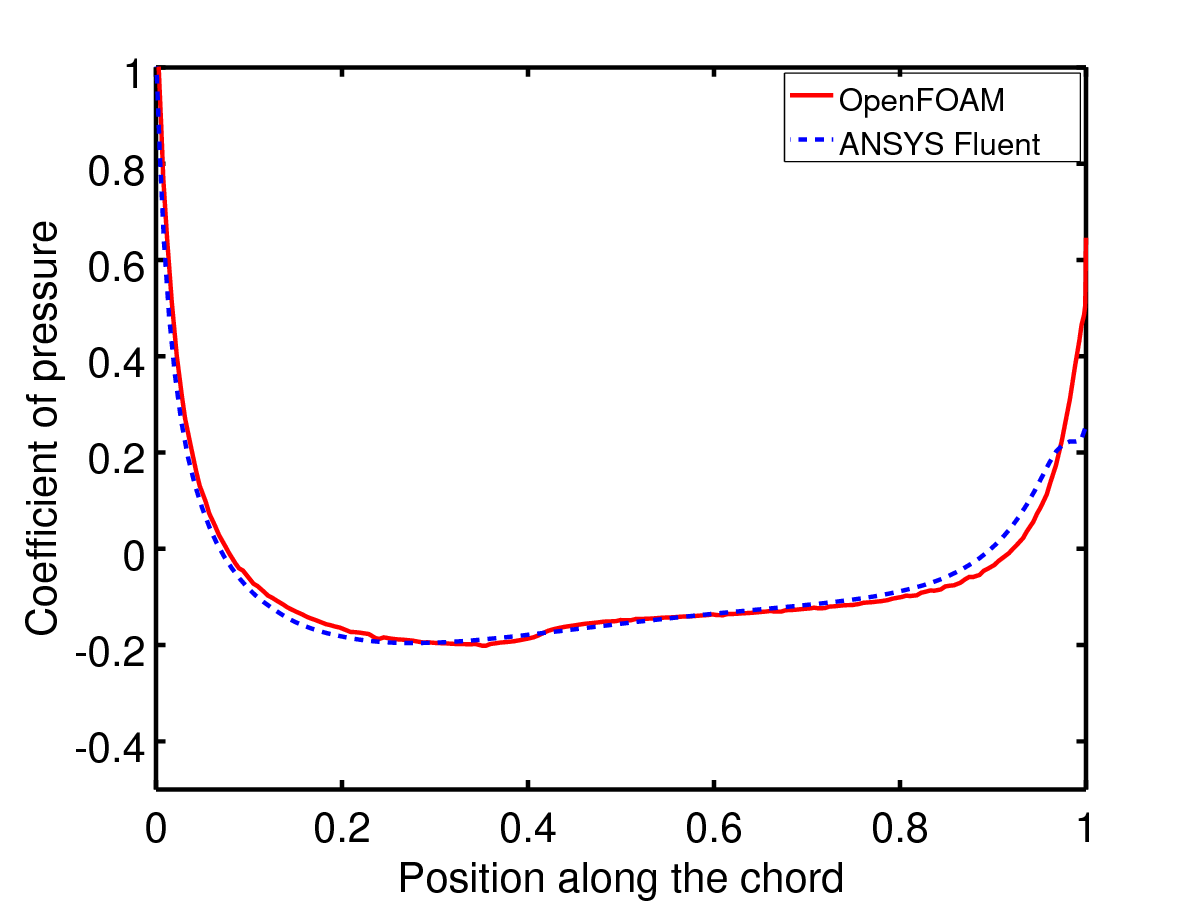
\includegraphics[width=300 pt]{rnd/NPL_cp.png}
	\caption{Comparison of OpenFOAM\textsuperscript{\textregistered} results with ANSYS\textsuperscript{\textregistered} \textit{Fluent} results for pressure distribution of NPL profile \cite{cheeseman2012}}
	\label{NPL fig} %      only if needed
\end{figure} 


Table \ref{NPL table} shows the comparison of $ C_{DV} $ obtained using OpenFOAM\textsuperscript{\textregistered} and ANSYS\textsuperscript{\textregistered} \textit{Fluent}.

\begin{table} [H]
	\centering
	\caption{\label{NPL table} Comparison of OpenFOAM\textsuperscript{\textregistered} results with ANSYS\textsuperscript{\textregistered} \textit{Fluent} for NPL shape}
	%	\begin{ruledtabular}
	\begin{tabular}{cccc}
		\hline \hline
		& OpenFOAM\textsuperscript{\textregistered} & ANSYS\textsuperscript{\textregistered} \textit{Fluent} & \% error \\ \hline \hline
		
		$ C_{DV} $ & 0.02598 & 0.02660 & 2.3    \\   \hline
	\end{tabular}
	%	\end{ruledtabular}
\end{table}

\pagebreak

\subsection{Grid Dependence study}
Since the solution is influenced by mesh size, three self similar grids with increasing number of grid points were considered. Table \ref{GridindependenceGNVR}, \ref{Grid independence study for Wang profile} and \ref{Grid independence study for NPL profile} compares the value for $C_{DV}$ obtained using OpenFOAM\textsuperscript{\textregistered} for GNVR \cite{Ram}, Wang \cite{Wangshape} and NPL\cite{cheeseman2012} shapes respectively.

\begin{table}[H]
	\caption{Grid Dependence study for GNVR shape}
	\label{GridindependenceGNVR} %      only if needed
	\centering
	%	\begin{ruledtabular}
	\begin{tabular}{ c c c c }
		\hline \hline
		& No. of cells & $C_{DV}$ using OpenFOAM\textsuperscript{\textregistered} & \% error change   \\ \hline \hline
		$ Coarse  $ & 198315  & 0.01565 & NA    \\  
		$ Fine $ & 646543  & 0.01555 & 0.6    \\  
		$ Very fine $ & 1444016  & 0.01572 & 1.1    \\ \hline	
	\end{tabular}
	%	\end{ruledtabular}
	
\end{table}

\begin{table}[H]
	\caption{Grid Dependence study for Wang shape}
	\label{Grid independence study for Wang profile} %      only if needed
	\centering
	%	\begin{ruledtabular}
	\begin{tabular}{  c c c c  }
		\hline \hline
		& No. of cells & $C_{DV}$ using OpenFOAM\textsuperscript{\textregistered} & \% error change \\ \hline \hline
		$ Coarse  $ & 1516763 & 0.02709  & NA    \\  
		$ Fine $ & 2494963 & 0.02597  & 10.2    \\  
		$ Very fine $ & 2808841 & 0.02496  & 7.9    \\  \hline	
	\end{tabular}
	%	\end{ruledtabular}
	
\end{table}


\begin{table}[H]
	\caption{Grid Dependence study for NPL shape}
	\label{Grid independence study for NPL profile} %      only if needed
	\centering
	%	\begin{ruledtabular}
	\begin{tabular}{  c  c c c }
		\hline \hline
		& No. of cells & $C_{DV}$ using OpenFOAM\textsuperscript{\textregistered} & \% error change \\ \hline \hline
		$ Coarse  $ & 220813 & 0.02709  & NA    \\  
		$ Fine $ & 1520195 & 0.02597  & 4.1    \\  
		$ Very fine $ & 2521622 & 0.02496  & 3.8    \\  \hline
	\end{tabular}
	%	\end{ruledtabular}
	
\end{table}



According to Suman et al. \cite{suman} if percentage changes compared to previous grid is $\le 5 \%$ then the value obtained from latest grid can be considered as the most accurate. From the above tables we may observe that for GNVR and NPL profiles, the percentage changes are $<$  5 \%, however for Wang profile, they are $>$5 \%. Thus, we can observe that the solution is nearly independent of grid size in all the cases.

\section{Observations \& Conclusions}

From the above results we can observe that OpenFOAM\textsuperscript{\textregistered} results match quite well with those obtained using commercial softwares like ANSYS\textsuperscript{\textregistered} \textit{Fluent} and other proprietary software like RANS \cite{suman}. The likely reasons for the minor differences in the values are as follows:
\begin{itemize}
	\item The results available in literature are 2D simulations using ANSYS\textsuperscript{\textregistered} \textit{Fluent} whereas in our case, they are 3D simulations using OpenFOAM\textsuperscript{\textregistered}.
	\item The mesh is different in the case of ANSYS\textsuperscript{\textregistered} \textit{Fluent} and OpenFOAM\textsuperscript{\textregistered}. OpenFOAM\textsuperscript{\textregistered}'s \textit{SnappyHexMesh} generates the mesh by splitting the cells of structured mesh.
	\item The values of some parameters (e.g., wall functions and wall boundary conditions) had to be assumed because they were not listed in the literature.
\end{itemize}
Apart from the above reasons, OpenFOAM\textsuperscript{\textregistered} solvers are also different from those of ANSYS\textsuperscript{\textregistered} \textit{Fluent}. Only a more detailed and systematic computational study and comparison with reliable experimental data can totally establish the efficacy of OpenFOAM\textsuperscript{\textregistered} w.r.t. ANSYS\textsuperscript{\textregistered} \textit{Fluent} and other proprietary codes.
In last three Chapters, we have discussed about geometry, mesh and solver. Now we have essential tools to carry out shape optimization. The methodology for optimization is discussed in next Chapter.


%%


%%% Local Variables: 
%%% mode: latex
%%% TeX-master: "../mainrep"
%%% End: 
